\documentclass[10pt]{article}
\usepackage[utf8]{inputenc}
\usepackage{amsmath,setspace,geometry}
\usepackage{amsfonts}
\usepackage[shortlabels]{enumitem}
%\usepackage[dvipdfmx]{hyperref,graphicx}
\usepackage{graphicx}
\usepackage{bbm}

\usepackage[colorlinks,citecolor=purple,urlcolor=blue,bookmarks=false,hypertexnames=true]{hyperref}
\usepackage[]{natbib} 
\bibpunct[:]{(}{)}{,}{a}{}{,}
\geometry{left = 1.0in,right = 1.0in,top = 1.0in,bottom = 1.0in}
%\onehalfspacing
% \usepackage{setspace}
\doublespacing
%\renewcommand{\baselinestretch}{0.3}
\usepackage[english]{babel}
\usepackage{float}
\usepackage{subfig}
\usepackage{booktabs}
\usepackage{pdfpages}
\usepackage{threeparttable}
\usepackage{lscape}
%\setstretch{1.2}
\newtheorem{assumption}{Assumption}
\newtheorem{definition}{Definition}
\newtheorem{example}{Example}
\newtheorem{lemma}{Lemma}

\title{Unified Dataset of Mergers in the Container Shipping Industry between 1966 and 2022: Transition of Importance of Tonnage Capacity and Geographical Proximity on Merger Decision}
\author{Suguru Otani\thanks{Department of Economics, Rice University. Email: so19@rice.edu}\quad  Takuma Matsuda\thanks{Faculty of Commerce, Takushoku University. Email: tmatsuda@ner.takushoku-u.ac.jp}}
\date{
First version: XXX\\
Current version: \today
}

\begin{document}

\maketitle

\begin{abstract}
We construct a novel unified panel dataset of mergers in the global container shipping industry between 1966 and 2022. Using the data, we construct a structural matching model \citep{fox2018qe} to describe the historical transition of the importance of tonnage capacity and geographical proximity on merger decisions. 
\textcolor{blue}{We find that XXX.}
\end{abstract} 

\vspace{0.1in}
\noindent\textbf{Keywords:} container shipping industry; exemption agreement; container crisis; 
\vspace{0in}


\section{Introduction}

Container shipping is a crucial component of global trade that has revolutionized the world. 
According to IHS Markit and Descartes Datamyne, container shipping accounts for $45.4 \%$ of amount-based imports to the U.S., $21.3 \%$ of amount-based exports from the U.S., and $10.12 \%$ of quantity-based world trade are shipped in 2021. 
Additionally, the container shipping industry offers a fascinating opportunity to explore industry dynamics such as entry, exit, and investment since the industry began global shipping operations in 1966 \citep{otani2023industry}. 
Despite its significance, like route-year-level prices and quantities dataset constructed by \cite{matsuda2022unified}, there is a lack of a unified dataset for the mergers in the container shipping industry, particularly for the years 1966 to 1990, which limits quantitative research during this period. 
This study provides a unified list of all mergers in the container shipping industry between 1966 and 2022.

Combining our new dataset with proprietary data, we conduct a structural analysis to quantify the relative importance of firm's age, size, and geographical proximity by applying a matching maximum score estimator \cite{fox2018qe}. 
\textcolor{blue}{It is anecdotally known that XXX. }



\subsection{Related literature}

This paper contributes to three strands of the literature, namely, empirical transferable utility (TU) matching, endogenous merger analysis, and recent industrial policy and antitrust studies in the shipping industry.

First, this paper contributes to the literature on empirical TU matching. 
The most related econometric model is \cite{fox2018qe}, whose model has been applied to other empirical topics such as banking merger \citep{akkus2015ms,chen2013ijio}, faculty room allocation \citep{baccara2012aer}, executive and firm matching \citep{pan2017determinants}, and buyer and seller relationships in the broadcast television industry \citep{stahl2016aer}. 
These papers have applied the matching maximum score estimator proposed by \cite{fox2010qe,fox2018qe} to two-sided many-to-many and one-to-one matching in a TU matching environment. 
We apply the approach to merger waves in the global container shipping industry from its inception.

Second, this paper contributes to the literature on endogenous merger analysis. Endogenous merger analysis in the industrial organization literature is divided into dynamic and static matching models. 
In terms of dynamic matching models, they follow \cite{gowrisankaran1999dynamic}.\footnote{\cite{stahl2011dynamic} was the first to estimate a merger activity model using a dynamic, strategic framework. \cite{jeziorski2014effects} estimated the sequential merger process to analyze ownership consolidation in the United States radio industry after the enactment of the Telecommunications Act of 1996. \cite{igami2019mergers} applied a stochastic sequential bargaining model to the merger processes of the hard disk industry. As the most recent paper, \cite{hollenbeck2020horizontal} enriched the Gowrisankaran-type dynamic endogenous merger model. With different dynamic approaches, \cite{nishida2015better} compared post-merger and pre-merger beliefs and equilibrium behaviors in a Markov perfect equilibrium in the Japanese retail chain industry. \cite{perez2015building} incorporated mergers as bidding games by incumbents and investigated the effect of the Reagan-Bush administration's merger policy on the reallocation of assets in the United States cement industry.} Conversely, using a static matching model, \cite{uetake2019entry} developed an empirical two-sided non-transferred utility matching model with externalities using moment inequalities and investigated the effect of entry deregulation on the ``with whom"-decisions of bank mergers by the Riegle-Neal Act. 
\cite{akkus2015ms} tackled the same Act with a different approach. 
They added transfer data and constructed a one-to-one matching model with transfer utility and found that merger value increased from cost efficiencies in overlapping markets, relaxing regulations, and the network effects exhibited by acquirer-target matching. 
Our paper follows \cite{akkus2015ms} and focuses on endogenous mergers in a single, static, large matching market for each regime and quantifies the relative importance of tonnage capacity and geographical proximity, which are the main economic forces driving firms to pursue mergers to gain cost efficiency in the shipping industry \citep{notteboom2004container}. 
In addition, we compare historical transitions of the relative importance of the variables.

Third, our paper contributes to the literature on recent industrial policy and antitrust studies in the shipping industry. \cite{jeon2022learning} studies the relationship between learning and investment in the container shipping industry between 2006 and 2014 and simulates counterfactual merger scenarios in which a merger occurred between top two firms that jointly account for over 35\% of total capacity in the industry.
\textcolor{blue}{[XXX]}



\section{Data and Industry Background}

We construct the data from combining the three data sources. 
The first data source is \textit{the Containerization International Yearbook} (CIY), which provides ship-level information between 1966 and 1990.
The second data source is IHS Markit data (IHS), which provides ship-level information between 1991 and 2005.
The third data source is \textit{Handbook of Ocean Commerce} (HB), which provides ship-level information between 2006 and 2022. 
We denote the period in the corresponding data as a \textit{regime}, that is, we observe three regimes.
Aggregating the ship-level data, we construct firm-level variables such as country name and tonnage capacity measured by the Twenty-foot Equivalent Unit (TEU). 
Finally, from institutional information, we manually construct a merger list that contains buyer names, seller names, and merger year, then merge the list with the firm-year-level variables. 

There are some remarks because we find that there are some inconsistencies such as a one-year lag and missing ship-level variables between these data sources and institutional facts. 
First, we fix the inconsistencies following the observations in the newer regime data. 
Second, we treat the firms not operating in the merged year as the firms that have a constant capacity level from the last active year in the merged year. % For example, Johnson Line was active in 1969-1972 but was merged in 1991.
Third, we treat mergers of some container shipping seller firms by non-container-shipping firms out of the industry as exits in the container shipping industry because it does not provide any information on buyer firms.
The final data regarding mergers is summarized in this section and used in empirical analysis in Section \ref{sec:empirical_analysis}.

\subsection{Industry Background}
We describe the industry background between 1966 and 2022 chronologically by focusing on firms' mergers. 
We classify the periods into three regimes, 1966-1990, 1991-2005, and 2006-2022. Each regime corresponds with the institutional background and data source.

\begin{table}[!htbp]
  \begin{center}
      \caption{Merger list: CIY (1966-1990)}
      \label{tb:merger_list_CIY} 
      
\begin{tabular}[t]{rllrl}
\toprule
ID & Seller & Buyer & Year & Type\\
\midrule
1 & Moore-McCormack Lines Inc & United States Lines & 1970 & acquisition\\
2 & OCL & P\&O Containers & 1986 & merger\\
3 & Franco-Belgian Services & Maersk & 1986 & merger\\
4 & Y-S Line & NLS & 1988 & merger\\
5 & Japan Line & NLS & 1988 & merger\\
6 & KSC & Hanjin & 1988 & merger\\
7 & Finland Steamship & Finnlines & 1990 & merger\\
8 & Atlanttrafik/Barber Blue Sea & Wilhelmsen Lines A/S & 1990 & merger\\
\bottomrule
\end{tabular}

  \end{center}\footnotesize
  %Note: 
\end{table} 

\begin{table}[!htbp]
  \begin{center}
      \caption{Merger list: IHS (1991-2005)}
      \label{tb:merger_list_IHS} 
      
\begin{tabular}[t]{llr}
\toprule
Seller & Buyer & Year\\
\midrule
IMC SHIPPING CO PTE LTD & IMC SHIPPING CO PTE LTD & 1993\\
BUSAN SHIPPING CO LTD & EUROSEAS LTD & 1994\\
CHINA MERCHANTS STEAM NAVIGATI & China Merchants Group & 1994\\
SVITZER AS & A P MOLLER & 1996\\
APL LTD & NEPTUNE ORIENT LINES LTD (NOL) & 1997\\
PRIMA SHIPMANAGEMENT SDN BHD & HALIM MAZMIN GROUP & 1999\\
FARRELL LINES INC & A P MOLLER & 2000\\
OOST ATLANTIC LIJN BV & ATLANTIC HORIZON GROUP & 2001\\
CYPRUS MARITIME CO LTD & CYPRUS SEA LINES SA & 2002\\
MISC BERHAD & Malaysia Shipping Corp Sdn Bhd & 2003\\
DANSK SUPERMARKED INVEST A/S & A P MOLLER & 2003\\
THE PENINSULAR AND ORIENTAL ST & A P MOLLER & 2004\\
EUROBULK LTD & EUROSEAS LTD & 2005\\
BARCLAY SHIPPING LTD & BARCLAY SHIPPING LTD & 2005\\
DELMAS & CMA CGM HOLDING & 2006\\
ROYAL P\&O NEDLLOYD NV & A P MOLLER & 2006\\
UNITED THAI SHIPPING CORP LTD & IMC SHIPPING CO PTE LTD & 2006\\
HORIZON LINES INC & MATSON NAVIGATION CO INC & 2006\\
EICKE SCHIFFAHRTS KG & EICKE SCHIFFAHRTS KG & 2006\\
CP SHIPS LTD & HAPAG-LLOYD AG & 2006\\
\bottomrule
\end{tabular}

  \end{center}\footnotesize
  %Note: 
\end{table} 

\begin{table}[!htbp]
  \begin{center}
      \caption{Merger list: HB (2006-2022)}
      \label{tb:merger_list_HB} 
      
\begin{tabular}[t]{rllrl}
\toprule
ID & Seller & Buyer & Year & Type\\
\midrule
1 & Cheng Lie & CMA-CGM & 2006 & acquisition\\
2 & Lloyd Triestino & Evergreen & 2006 & merger\\
3 & Norasia & CSAV & 2006 & acquisition\\
4 & MacAndrews & CMA-CGM & 2007 & acquisition\\
5 & Lufeng & Sinotrans & 2008 & merger\\
6 & NEW ONTO SHIPPING & GOTO Shipping International Ltd & 2010 & merger\\
7 & TSK & NYK & 2010 & merger\\
8 & China Navigation & Swire & 2011 & acquisition\\
9 & CCNI & Maersk & 2015 & acquisition\\
10 & CSAV & Hapag-Lloyd & 2015 & acquisition\\
11 & China Shipping & COSCO & 2016 & merger\\
12 & Shanghai Puhai Shipping & COSCO & 2016 & merger\\
13 & UASC & Hapag-Lloyd & 2017 & acquisition\\
14 & KLINE & Ocean Network Express & 2018 & merger\\
15 & MOL & Ocean Network Express & 2018 & merger\\
16 & NYK & Ocean Network Express & 2018 & merger\\
17 & APL & CMA-CGM & 2017 & acquisition\\
18 & Hamburg Sud & Maersk & 2018 & acquisition\\
\bottomrule
\end{tabular}

  \end{center}\footnotesize
  %Note:
\end{table} 

\paragraph{1966-1990} 

Table \ref{tb:merger_list_CIY} summarizes all mergers based on CIY between 1966 and 1990.\footnote{In 1964, the Japanese ocean shipping industry experienced consolidation induced by the government, and 95 firms were merged into six large groups. \cite{otani2021estimating} investigates the event by a structural matching model.}
This period involves a collusive and competitive environment with shipping conferences that are explicit and cartels globally allowed. 
The period is studied in \cite{matsuda2022unified} and \cite{otani2023industry} in detail.
The period is divided into the collusive (1966-1983) and competitive (1984-1990) periods due to the U.S. Shipping Act of 1984.
In the collusive period between 1966 and 1983, a single merger occurred in 1970 (Moore-McCormack Lines Inc merged by United States Lines). % and 1972 (Johnson Line merged by NA).
In the competitive period between 1984 and 1990, two mergers occurred in 1986, three mergers occurred in 1988, and two mergers occurred in 1990. 
\textcolor{blue}{Anecdotally, mergers in the period are driven by XXX}
% Background
% What mergers?

\paragraph{1991-2008}

Table \ref{tb:merger_list_IHS} summarizes all mergers based on IHS between 1991 and 2005.
\textcolor{blue}{Anecdotally, mergers in the period are driven by XXX}
% Background
% What mergers?




\paragraph{2009-2022}

% Background
% What mergers?

Table \ref{tb:merger_list_HB}





% (Need to validate with NYK aggregate TEU data just for confirmation.)

\subsection{Descriptive statistics}

Table \ref{tb:summary_statistics} shows summary statistics of buyer and seller firms in all realized merger cases between 1966 and 2022. 
We construct firm-level variables such as the firm's age in the global container shipping industry and size measured by TEU in the merger year. 
We normalized these variables from 0 (minimum age) to 1 (maximum age) in each regime for comparison across regimes.
First, we find that the mean of normalized firms' age decreases from 0.84 in the 1966-1990 period to 0.51 in the 2006-2022 period. This implies that mergers are likely to occur between relatively younger firms in recent years.
Second, the mean of normalized firms' size decreases from 0.23 in the 1966-1990 period to 0.08 in the 2006-2022 period. 
This implies that mergers are likely to occur between relatively smaller firms in recent years, although the firm's absolute size increases exponentially. 
Note that we treat new entrant firms buying incumbent firms as firms whose age and size are zero so that the above findings capture that the number of entries by mergers increases.
Figure \ref{fg:size_cdf} illustrates XXX.


\begin{table}[!htbp]
  \begin{center}
      \caption{Summary statistics of buyer and seller firms}
      \label{tb:summary_statistics} 
      \subfloat[CIY (1966-1990)]{
\begin{tabular}[t]{lrrrrr}
\toprule
  & N & mean & sd & min & max\\
\midrule
Age (Normalized) & 16 & 0.84 & 0.24 & 0.23 & 1.00\\
Size TEU (Normalized) & 16 & 0.23 & 0.29 & 0.01 & 1.00\\
\bottomrule
\end{tabular}
}\\
      \subfloat[IHS (1991-2005)]{
\begin{tabular}[t]{lrrrrr}
\toprule
  & N & mean & sd & min & max\\
\midrule
Age (Normalized) & 40 & 0.58 & 0.39 & 0.00 & 1.00\\
Size TEU (Normalized) & 40 & 0.11 & 0.22 & 0.00 & 1.00\\
\bottomrule
\end{tabular}
}\\
      \subfloat[HB (2006-2022)]{
\begin{tabular}[t]{lrrrrr}
\toprule
  & N & mean & sd & min & max\\
\midrule
Age (Normalized) & 60 & 0.51 & 0.30 & 0.11 & 1.00\\
Size TEU (Normalized) & 60 & 0.08 & 0.19 & 0.00 & 1.00\\
\bottomrule
\end{tabular}
}
      
  \end{center}\footnotesize
  %Note:
\end{table} 

\begin{figure}[!ht]
\begin{center}
  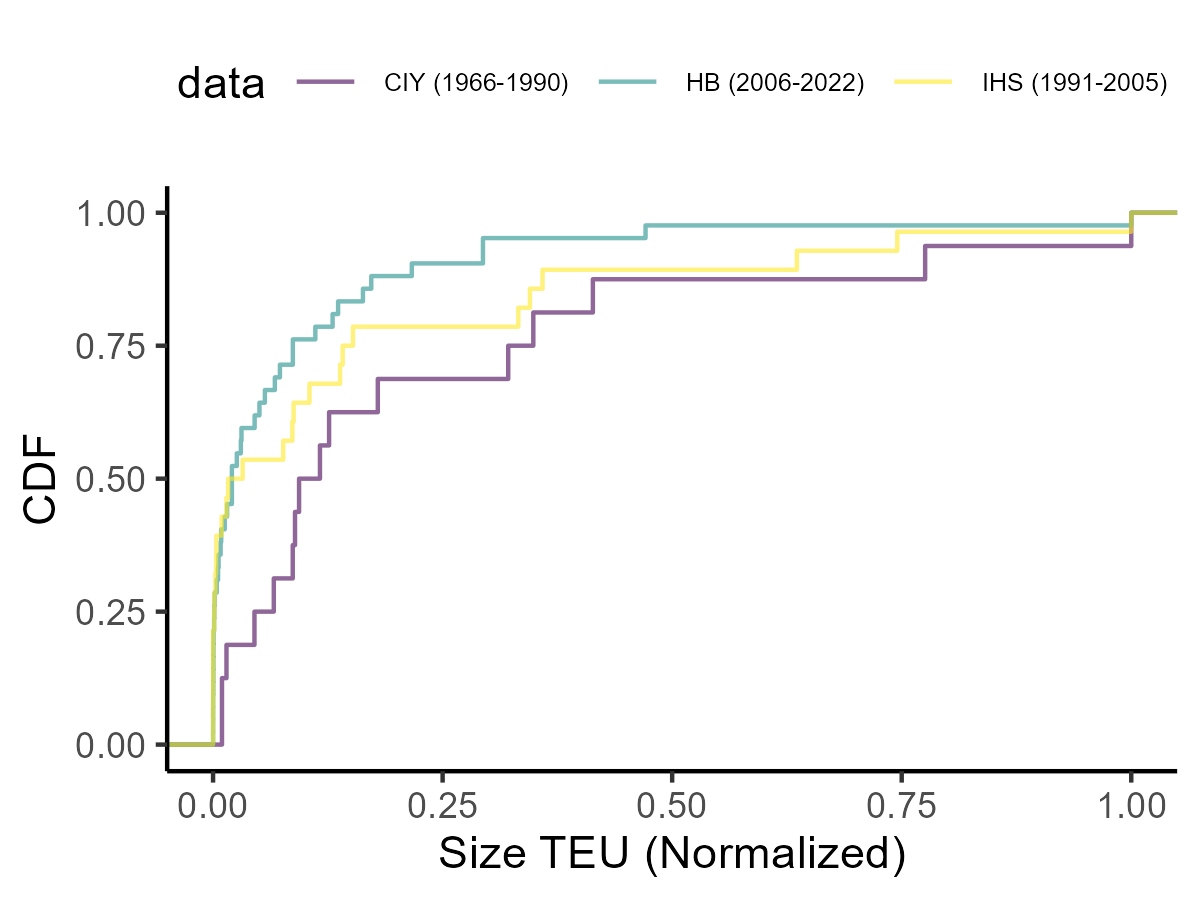
\includegraphics[width = 0.45\textwidth]
  {figuretable/normalized_size_cdf.png}
  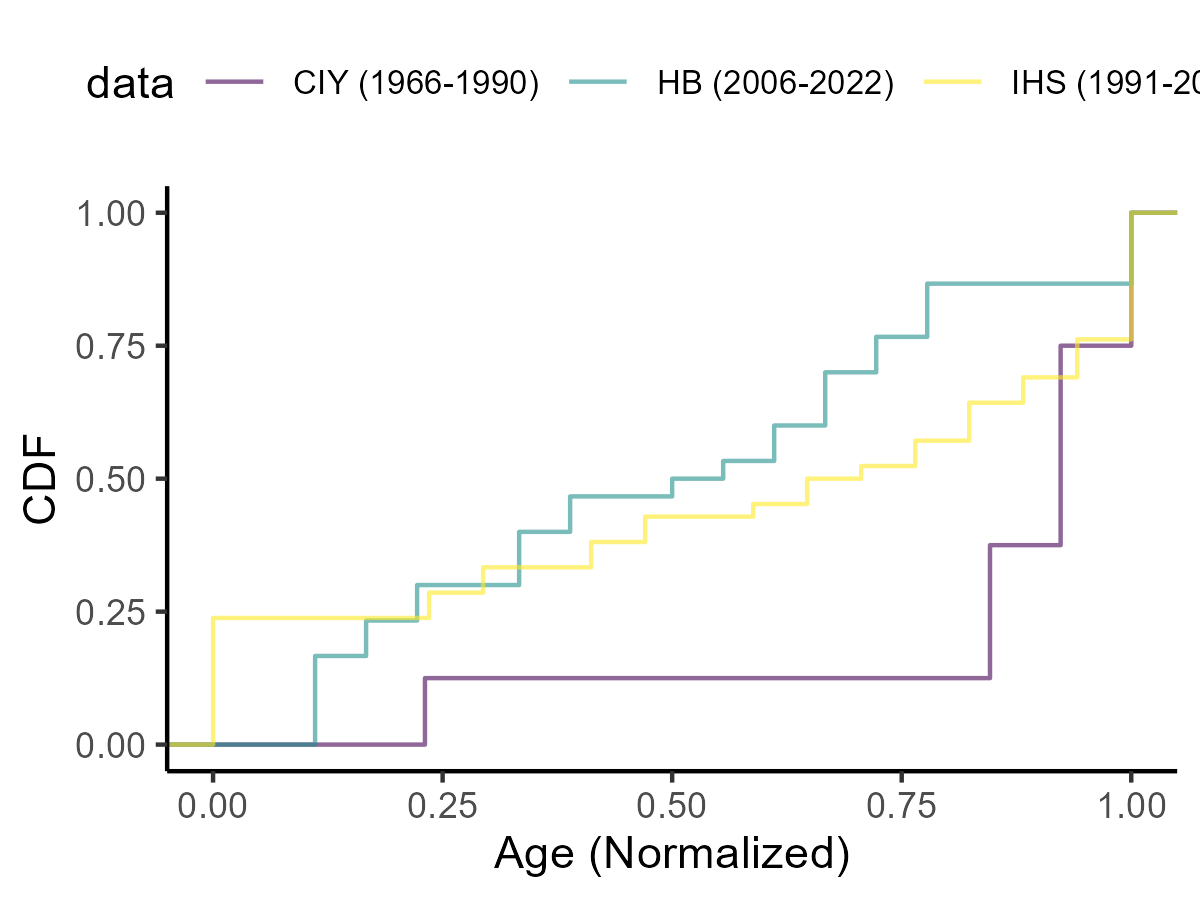
\includegraphics[width = 0.45\textwidth]
  {figuretable/normalized_age_cdf.png}
  \caption{Distributions of normalized firm's size and age for each regime}
  \label{fg:size_cdf}
  \end{center}
\footnotesize
   %Note: 
\end{figure}

\begin{figure}[!ht]
\begin{center}
  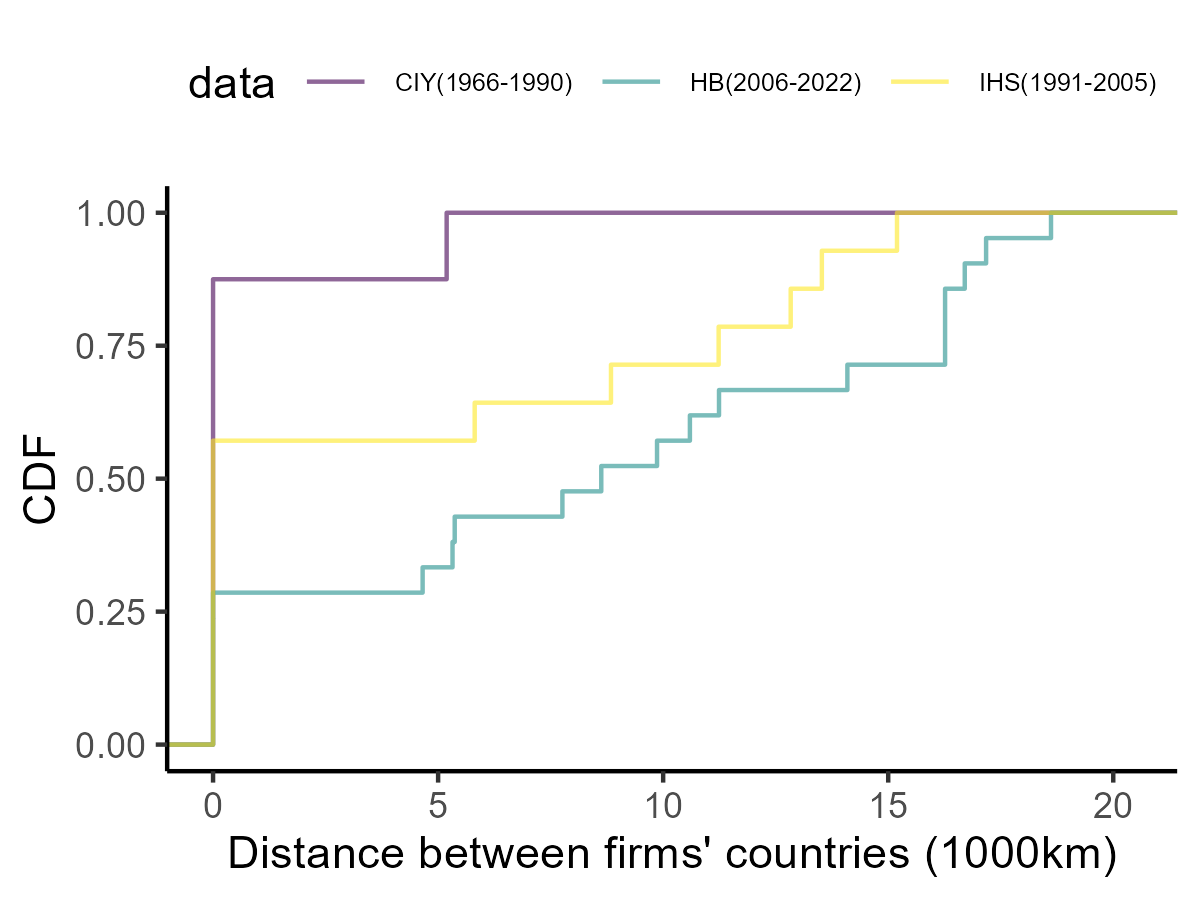
\includegraphics[width = 0.7\textwidth]
  {figuretable/distance_cdf.png}
  \caption{Distributions of realized buyer-seller-level distances for each regime}
  \label{fg:distance_cdf}
  \end{center}
\footnotesize
   %Note: 
\end{figure}


Figure \ref{fg:distance_cdf} illustrates distributions of realized buyer-seller-level distances. 
We find that almost all mergers between 1966 and 1990 involve buyer and seller firms in the same country. 
Although the share of mergers in the same country is more than 40 \% in the whole period, the share of mergers of firms between countries separated by distance increases in recent years. 
This implies that the reason why mergers occur seems to change from domestic one to global one due to the prosperity and expansion of international container transport.

These tables and figures provide some intuition that mergers are likely to involve relatively younger and smaller firms in more distant countries in recent years. 
However, disentangling the relative importance of each variable with limited data needs a more sophisticated structural model.
In Section \ref{sec:empirical_analysis}, we construct a structural matching model to quantify the relative importance of each variable and compare the transition across regimes.




\section{Empirical analysis}\label{sec:empirical_analysis}

Our objective is to quantify the assortativeness of observed characteristics  for each regime and compare the levels across regimes. 
We employ a matching maximum score estimator developed by \cite{fox2018qe}, which is one of the most well-known methods for measuring matching assortativeness.

For exposition, we model mergers in each regime as a two-sided one-to-one transferable matching game in a single market. Let $\mathcal{N}_b$ and $\mathcal{N}_s$ be the sets of potential finite buyers and sellers respectively. Let $b=1,\cdots,|\mathcal{N}_b|$ be buyer firms and let $s=1,\cdots,|\mathcal{N}_s|$ be seller firms where $|\cdot|$ is cardinality. Let $\mathcal{N}_{b}^{m}$ denote the set of ex-post matched buyers and $\mathcal{N}_{b}^{u}$ denote that of ex-post unmatched buyers such that $\mathcal{N}_b= \mathcal{N}_{b}^{m}\cup\mathcal{N}_{b}^{u}$ and $\mathcal{N}_{b}^{m}\cap\mathcal{N}_{b}^{u}=\emptyset$. For the seller side, define $\mathcal{N}_{s}^{u}$ and $\mathcal{N}_{s}^{m}$ as the set of ex-post matched and unmatched sellers such that $\mathcal{N}_s= \mathcal{N}_{s}^{m}\cup\mathcal{N}_{s}^{u}$ and $\mathcal{N}_{s}^{m}\cap\mathcal{N}_{s}^{u}=\emptyset$. Let $\mathcal{M}^m$ be the sets of all ex-post matched pairs $(b,s)\in\mathcal{N}_{b}^{m}\times \mathcal{N}_{s}^{m}$. Let $\mathcal{M}$ denote the set of all ex-post matched pairs $(b,s)\in\mathcal{M}^{m}$ and unmatched pairs $(\tilde{b},\emptyset)$ and $(\emptyset,\tilde{s})$ for all $\tilde{b}\in \mathcal{N}_b^u$ and $\tilde{s}\in \mathcal{N}_s^u$ where $\emptyset$ means a null agent generating unmatched payoff. 

Each firm can match at most one agent on the other side, so  $|\mathcal{N}_b^{m}|=|\mathcal{N}_s^{m}|$. The matching joint production function is defined as $f(b,s)=V_b(b,s)+V_s(b,s)$ where $V_b:\mathcal{M}\rightarrow \mathbb{R}$ and $V_s:\mathcal{M}\rightarrow \mathbb{R}$. The net matching values for buyer $b$ and seller $s$ are defined as $V_b(b,s)=f(b,s)-p_{b,s}$ and $V_s(b,s)+p_{b,s}$, where $p_{b,s}\in \mathbb{R}_{+}$ is the equilibrium merger price paid to seller firm $s$ by buyer firm $b$ and $p_{b\emptyset}=p_{\emptyset s}=0$. For scale normalization, we assume $V_b(b,\emptyset)=0$ and $V_s(\emptyset,s)=0$ for all $b\in \mathcal{N}_b$ and $s\in \mathcal{N}_s$. Each buyer maximizes $V_b(b,s)$ across seller firms, whereas each seller maximizes $V_s(b,s)$ across buyer firms. 

The stability conditions for buyer firm $b \in \mathcal{N}_b$ and seller firm $s \in \mathcal{N}_s$ are as follows:
\begin{align}
    V_b(b,s) &\ge V_b(b,s') \quad \forall s' \in \mathcal{N}_s \cup \emptyset,s'\neq s,\label{eq:stability_ineq}\\
    V_s(b,s) &\ge V_s(b',s) \quad \forall b' \in \mathcal{N}_b\cup \emptyset,b'\neq b.\nonumber
\end{align}

Based on Equation \eqref{eq:stability_ineq} and equilibrium price conditions $p_{b',s}\le p_{b,s}$ and $p_{b,s'}\le p_{b',s'}$ in \cite{akkus2015ms}, we construct the inequalities for matches $(b,s)\in \mathcal{M}$ and $(b',s')\in \mathcal{M}, (b',s')\neq(b,s)$ as follows:
\begin{align}
    f(b,s)-f(b,s')&\ge p_{b,s}-p_{b,s'}\ge p_{b,s}-p_{b',s'},\label{eq:pairwise_stable_ineq}\\
    f(b',s')-f(b',s)&\ge p_{b',s'}-p_{b',s}\ge p_{b',s'}-p_{b,s},\nonumber\\
    V_s(b,s)-V_s(b',s)&\ge 0,\nonumber\\
    V_{s'}(b',s')-V_s(b,s')&\ge 0,\nonumber
\end{align}
where $p_{b',s}$ and $p_{b,s'}$ are unrealized equilibrium merger prices that cannot be observed in the data. The last two inequalities cannot be derived from the data because the researchers cannot observe how the total matching value $f(b,s)$ is shared between buyer $b$ and seller $s$.

\cite{fox2018qe} proposes a maximum score
estimator using the above inequalities. The maximum score estimator is consistent if the model satisfies a rank order property, i.e., the probability of observing matched pairs is larger than the probability of observing swapped matched pairs. We specify $f(b,s)$ as a parametric form $f(b,s|X,\beta)$ where $X$ is a vector of observed characteristics of all buyers and sellers and $\beta$ is a vector of parameters. As observed characteristics $X$, we use the age and total tonnage of each firm and the geological location of the flag country at merger timing.


Given $X$, one can estimate $\beta$ by maximizing the following objective function:
\begin{align}
    Q(\beta)=\sum_{(b,s)\in \mathcal{M}} \sum_{(b',s')\in \mathcal{M},(b',s')\neq (b,s)} \mathbbm{1}[f(b,s|X,\beta)+ f(b',s'|X,\beta)\ge f(b,s'|X,\beta)+f(b',s|X,\beta)]\label{eq:score_function}
\end{align}
where $\mathbbm{1}[\cdot]$ is an indicator function.

In our empirical application, we use the standardized firm's age and size and match-level distance variables in the observed characteristics.


\section{Results}

Table \ref{tb:maximum_score_estimate}

\begin{table}[!htbp]
  \begin{center}
      \caption{Matching maximum score estimation}
      \label{tb:maximum_score_estimate} 
      
\begin{tabular}[t]{lcc}
\toprule
Regime & 1966-1990 & 2005-2022\\
Standardized Firm age & 1 & 1\\
Standardized Firm-year-level TEU & {}[3e-04,0.0331] & {}[0.0019,0.1197]\\
\% of correct matches & 0.9643 & 0.9715\\
\bottomrule
\end{tabular}

  \end{center}\footnotesize
  Note: 
\end{table} 

\section{Counterfactual}

Table XXX.


\section{Conclusion}

\bibliographystyle{aer}
\bibliography{container_merger_data_bib}


\end{document}